\section{Crowd-Shared Wireless Mesh Networks}
\label{sec:architecture}

\begin{figure}[t]
\begin{center}
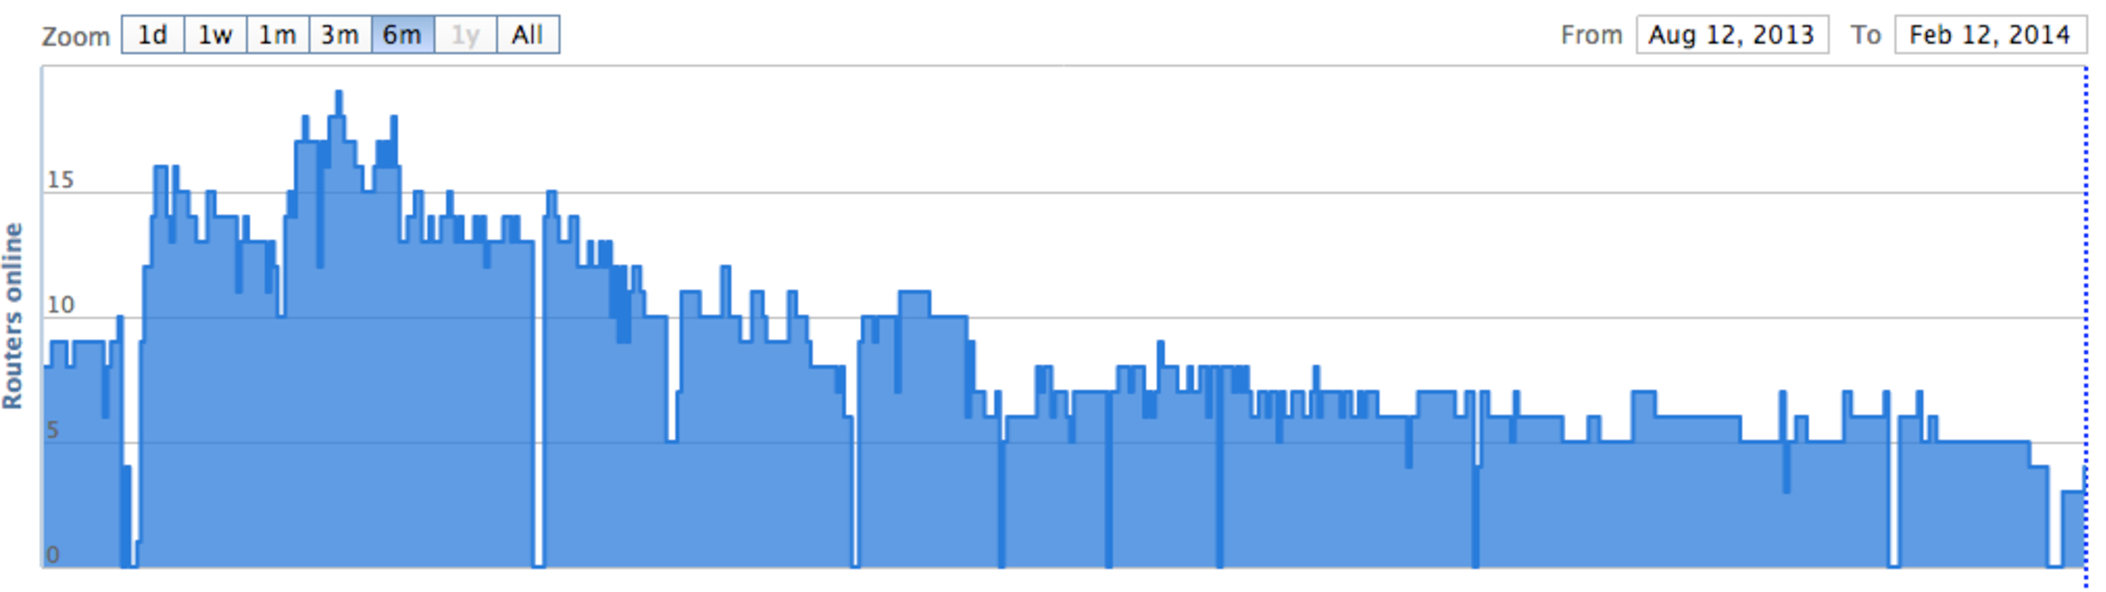
\includegraphics[width=1\linewidth]{paws-avail.pdf}  
\caption{PAWS routers availability.}
\label{fig:paws-avail}
\end{center}
\end{figure}

The underlying problem with PAWS or any crowd-shared network is that they serve as single point of Internet access to guest users within the coverage of the wireless router and hence, they have no provision to extend the coverage when no bandwidth is being shared. Based on our experience from the trial PAWS deployment, PAWS routers were always not available for certain periods, because sharers needed all the bandwidth of their broadband connection or due to other reasons, such as economic constraints placed on home users in underprivileged areas where they are forced to conserve energy by turning off the routers at nights. In this respect, Fig. \ref{fig:paws-avail} presents a six-month view of the PAWS routers status (available/unavailable) logs demonstrating that not a single router was available continuously over the entire duration. These observed user behaviors entail significant challenges for the successful adoption of PAWS. 

\subsection{Crowd-Shared WMN Management}
\label{architecture:management}

A potential solution to this problem is to extend the PAWS network as a crowd-shared WMN. Such a network would allow home network users to share part of their own broadband connection to the public for free while also connected to each other as a WMN providing extended coverage (Fig. \ref{fig:wmn}). Extending PAWS to a crowd-shared WMN departs from the norm: multiple users from different ISPs form part of the WMN to provide free Internet connectivity, while most wireless community WMNs today are operated by a single organization. This raises important questions regarding the operation, configuration, and management of crowd-shared WMNs.  

\begin{figure}[t]
\begin{center}
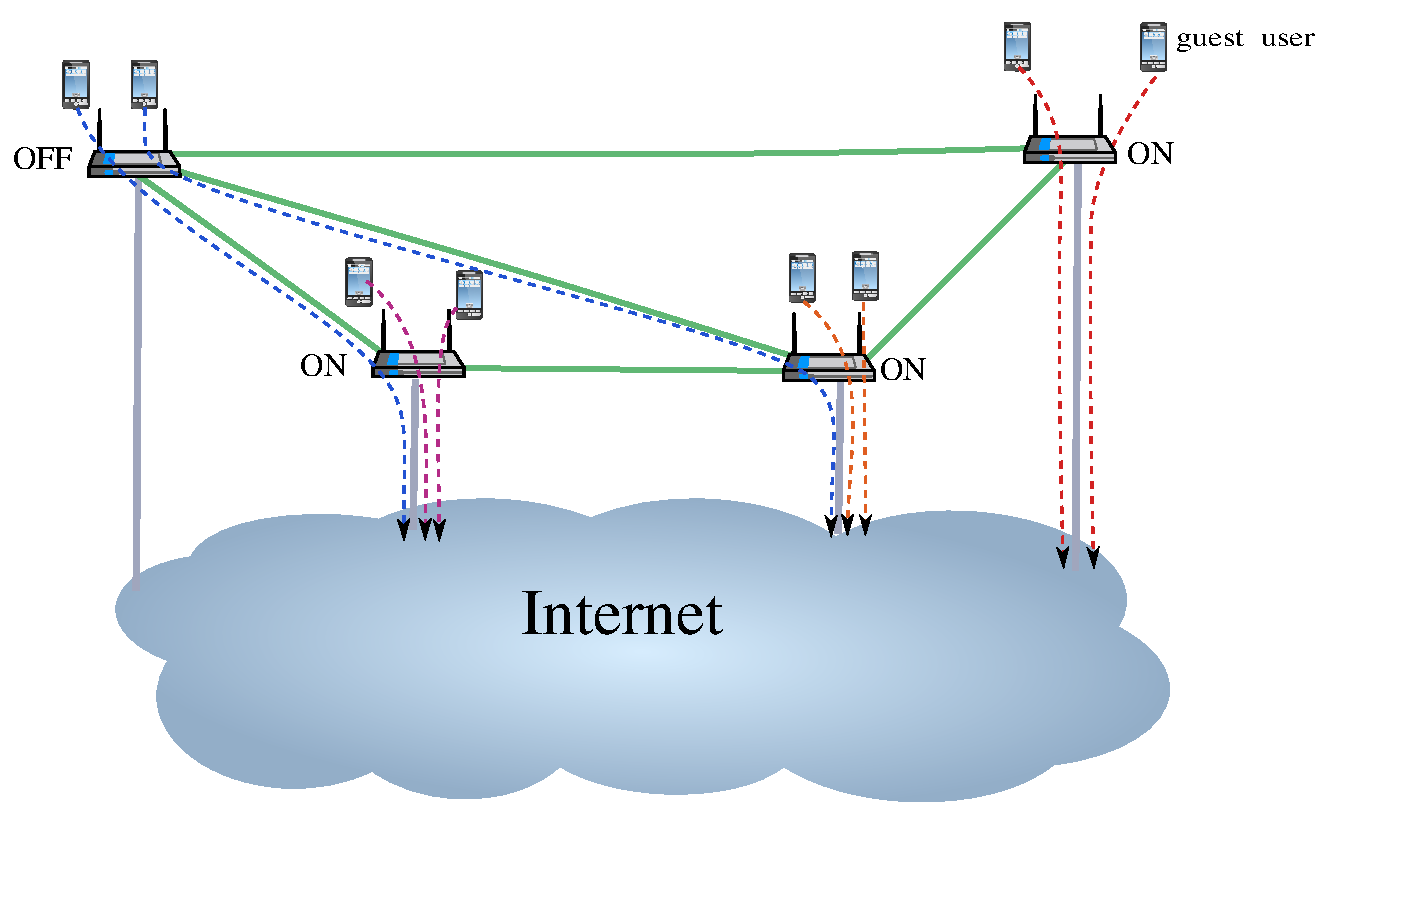
\includegraphics[width=1\linewidth]{flow_redirection.pdf}  
\caption{Crowd-shared WMN for public Internet access.}
\label{fig:wmn}
\end{center}
\end{figure}

SDN can facilitate the management and operation of wireless networks at large scale. Leveraging on SDN's centralized control and network-wide visibility, the management and operation of a crowd-shared WMN can be outsourced to a third party. In \cite{EWSDN}, we describe a holistic approach of coupling both social and economic incentives in designing future networks allowing the extension of the stakeholder value chain to include more than the two traditional parties (consumer and Internet service provider). Such an approach would provide opportunities for non-governmental organizations and local governments (driven by social goals rather than economic) to become virtual network operators. Enabling a third party to federate such wireless home networks would reduce the operating expenditures for network operators as well as enable new economic models for revenue creation from currently underutilized infrastructures. In particular, we rely on SDN to create the notion of Virtual Public Networks (VPuN), i.e., crowd-shared home networks created, deployed and managed through an evolutionary SDN control abstraction \cite{EWSDN}. Although originally intended for crowd-shared wireless networks such as PAWS, VPuN can also facilitate management of crowd-shared WMNs, enabling resource pooling across multiple home broadband connections based on the prevailing network conditions and usage sharing patterns. 

\subsection{Traffic Redirection}
\label{architecture:redirection}

To take advantage of the extended coverage provided by a WMN, we develop and evaluate techniques for the redirection of guest user traffic during the periods that the home user does not permit the sharing of his broadband connection. In this case, Internet is accessed through the router of another home network where sharing is allowed. 

In the following, we present an algorithm for the assignment of the gateway and the path over which the traffic will be redirected through the WMN. We assume that this algorithm will be executed by a SDN controller which has knowledge of the WMN topology and utilization as well as the broadband network utilization and user sharing policies. 

We represent the WMN as a weighted undirected graph $G = (N, L)$, where $N$ is the set of nodes and $L$ is the set of links between nodes of the set $N$. Each node $n_i$ is associated with an Internet access link whose available bandwidth capacity is denoted by $C(n_i)$. Each link $l_{ij} \in L$ between two nodes $n_i$ and $n_j$ is associated with the available bandwidth capacity $C(l_{ij})$. Let $P_{ij}$ denote the set of paths in the network $G$, between the pair of nodes $n_i$ and $n_j$. The available bandwidth capacity $C(p)$ associated to a path $p \in P_{ij}$ is given by the minimal residual bandwidth of the links along the path:

\begin{equation}
C(p) = \min_{l_{ij} \in p} C(l_{ij}))
\end{equation}

%Let $M$ denote a link capacity matrix associated to the graph $G$, such that $M$=[$C(l_{ij})$] is the available bandwidth capacity matrix for links $l \in L$ between nodes $n_i$ and $n_j$, where $1 \leq i,j \leq |N|$.

We further represent a flow demand for a guest user with the tuple $d = (n_u, r)$, where $n_u \in N$ is the node where the guest user device has been attached and $r$ denotes the flow rate. We use $D$ to represent the set of flow demands that have arrived in the system.

\algsetup{indent=0em}
\begin{algorithm}[htbp]
  \caption{Gateway and Path Assignment}
  \label{assignment}
  \begin{algorithmic}
  \small
    \STATE \textbf{Inputs}: $G = (N, L), D$
    \vspace{2mm}
    \STATE  SORT($D$)
    \vspace{0.7mm}
    \FOR{each $d \in D$}
    \vspace{0.7mm}
    \STATE \hspace{0.4cm} $search \leftarrow$ true
    \vspace{0.7mm}
    \STATE \hspace{0.4cm} $M \leftarrow \{N \setminus {n_u}\}$
    \vspace{0.7mm}
    \STATE \hspace{0.4cm} \textbf{while} ($search$)
    \vspace{0.7mm}
    \STATE \hspace{0.8cm} $g \leftarrow argmax_{i \in M} C(n_i)$
    \vspace{0.7mm} 
    \STATE \hspace{0.8cm} \textbf{for} each $p \in P_{ug}$
    \vspace{0.7mm}
    \STATE \hspace{1.2cm} \textbf{if} $C(p) < r$ \textbf{then}
    \vspace{0.7mm}
    \STATE \hspace{1.6cm} $P_{ug} \leftarrow P_{ug} \setminus {p}$
    \vspace{0.7mm}
    \STATE \hspace{1.2cm} \textbf{end if}
    \vspace{0.7mm}
    \STATE \hspace{0.8cm} \textbf{end for}
    \vspace{0.7mm}
    \STATE \hspace{0.8cm} \textbf{if} $P_{ug} = \emptyset$ \textbf{then}
    \vspace{0.7mm}
    \STATE \hspace{1.2cm} $M \leftarrow M \setminus {n_g}$
    \vspace{0.7mm}
    \STATE \hspace{0.8cm} \textbf{else}
    \vspace{0.7mm}
    \STATE \hspace{1.2cm} $search \leftarrow$ false
    \vspace{0.7mm}
    \STATE \hspace{0.8cm} \textbf{end if}
    \vspace{0.7mm}
    \STATE \hspace{0.4cm} \textbf{end while}
    \vspace{0.7mm}
    \STATE \hspace{0.4cm} $n_g \leftarrow$ gateway \hspace{0.2cm} // gateway assignment
    \vspace{0.7mm}
    \STATE \hspace{0.4cm} $p \leftarrow \mathrm{SP} (P_{ug})$ \hspace{0.3cm} // path assignment
    \vspace{0.7mm}
    \ENDFOR
  \end{algorithmic}
\end{algorithm}

The algorithm assigns a gateway and the best path to each flow demand from the set $D$. The algorithm is executed whenever there is insufficient shared bandwidth in the local home network. Initially the flow demands are sorted based on the flow rate in decreasing order. For each flow demand, the algorithm selects the home router with the highest bandwidth in its access link (i.e., $C(n_i)$). Subsequently, the algorithm identifies the set of paths between the local home router ($n_u$) and the assigned gateway ($n_g$) that satisfy the flow rate requirement (Equation 1). In case there is no such path, the algorithm performs another iteration for the selection of the gateway, excluding the previously selected home router. Otherwise, the shortest among these paths is being identified based on the number of hops (SP function in the algorithm). This eventually designates the path for the traffic redirection through the WMN.

This algorithm carries out the gateway assignment based on the available shared bandwidth of the home routers in the crowd-shared network. Although this can pool resources from all home networks where sharing is permitted achieving efficient utilization of the shared bandwidth, guest user traffic may have to traverse multiple hops in the WMN. This can lead to latency inflation, delay variation and in general, unpredictable performance. To mitigate this, we also use a variant of this algorithm by introducing a threshold in the number of hops between the local home router and the assigned gateway. For example, setting the threshold to 1, restricts the gateway assignment to one of the next-hop routers with sufficient shared bandwidth.


